\documentclass[]{beamer}
%\documentclass[handout]{beamer}
%\documentclass[handout,draft]{beamer}

% Preambulo
% Paquetes para usar bien el idioma español
\usepackage[spanish,es-tabla]{babel}
\selectlanguage{spanish}
\usepackage[utf8]{inputenc}

% Paquetes para usar mejores imagenes
\usepackage{graphicx}

% Paquetes para links y tabla de contenidos en el PDF
\usepackage{hyperref}
\hypersetup{colorlinks=true,allcolors=blue}
%\usepackage{hypcap}

% Paquetes para mejores tablas
\usepackage{booktabs}

% Mejor matematica
\usepackage{amsmath}

% Fuentes de las imagenes
\usepackage[absolute,overlay]{textpos}

% Paquete captions
\usepackage[justification=centering,labelformat=empty,labelsep=none]{caption}

% Opciones para ticks
\usepackage{tikz}
\usetikzlibrary{shapes,arrows,positioning}

\tikzstyle{decision} = [diamond, draw, fill=blue!20, text width=4em, text badly centered, node distance=2cm, inner sep=0pt,on grid]
\tikzstyle{block} = [rectangle, draw, fill=blue!20, text width=8em, text centered, rounded corners, minimum height=2em,on grid]
\tikzstyle{line} = [draw, -latex]

% Citas bibliograficas
\usepackage[backend=biber]{biblatex}
\renewcommand{\footnotesize}{\tiny}
\addbibresource{biblio.bib}

% Mejoro las captions
\setbeamertemplate{caption}{\raggedright\insertcaption\par}

\setbeamertemplate{caption}{%
\begin{beamercolorbox}[wd=0.85\paperwidth, sep=.2ex]{block body}\insertcaption%
\end{beamercolorbox}%
}


% Sacar barra de navegacion
\setbeamertemplate{navigation symbols}{}%remove navigation symbols

% Transparencias en items
\setbeamercovered{transparent}

% Estilo de diapositivas
% \usetheme{Boadilla}
\usecolortheme{whale}
\usecolortheme{orchid}


\title{Herramientas de Teledetección Cuantitativa\\{\small Clase 7}}
\author{Francisco Nemi\~na}
\institute{Unidad de Educación y Formación Masiva \\ Comisión Nacional de
Actividades Espaciales}
%\institute[Inst.]{
\includegraphics[height=1cm]{Figures/logosopi.png}\phantom{pepe} 
\includegraphics[height=1cm]{Figures/2mp.png}\phantom{pepe} 
\includegraphics[height=1cm]{Figures/conae.png}}
\date{}
%\titlegraphic{
%\includegraphics[height=1cm]{IMAGENES/minplan.png}\phantom{1}
%
\includegraphics[height=1cm]{IMAGENES/conae.png}\phantom{1}
%
\includegraphics[height=1cm]{IMAGENES/sopi.png}}

\logo{
\includegraphics[height=0.7cm]{imagenes/sopi.png}}

\AtBeginSection[]
{
\begin{frame}
\frametitle{Esquema de presentación}
\tableofcontents[currentsection]
\end{frame}
}


\begin{document}
\begin{frame}
    \maketitle
\end{frame}

\section{Introducción}
\subsection{Nociones básicas}
\begin{frame}{\subsecname}
\begin{block}{Objetivo de la validación}
  Lo que esperamos es asignarle a nuestro mapa temático un cierto grado de confianza a partir de datos medidos en el terreno.
\end{block}
\end{frame}

\begin{frame}{\subsecname}
  \begin{figure}
  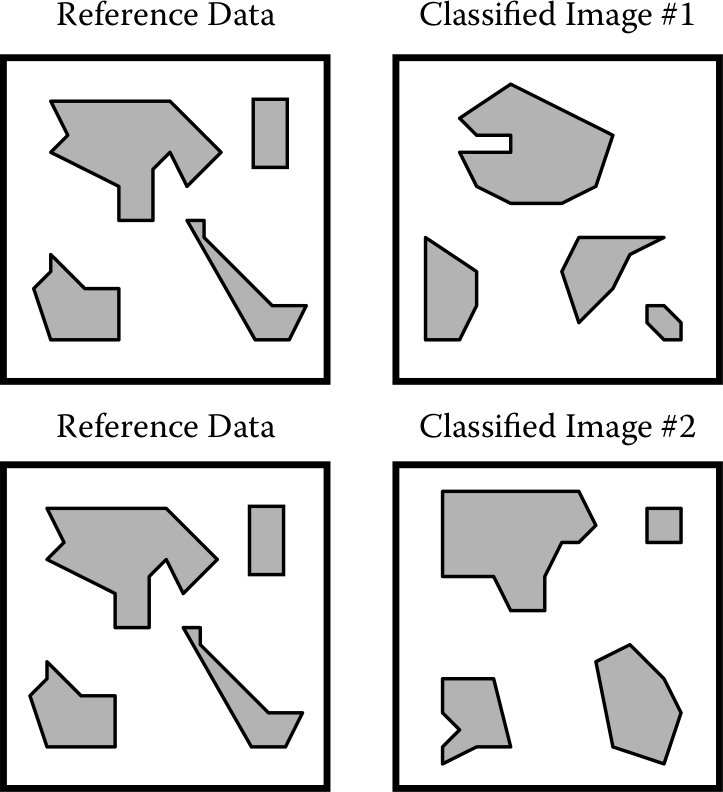
\includegraphics[width=0.5\textwidth]{imagenes/valid.png}
  \caption{Ejemplo de datos de referencia contra un mapa temático.\footfullcite{congalton2008assessing}}
  \end{figure}
\end{frame}
%--- Next Frame ---%

\begin{frame}{\subsecname}
  \begin{figure}
  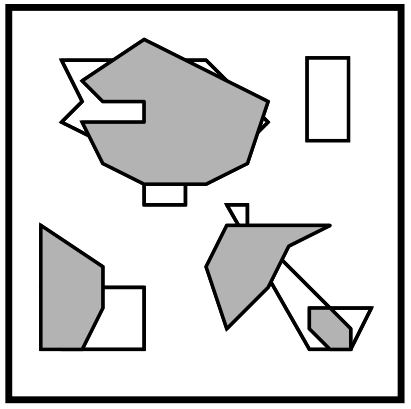
\includegraphics[width=0.4\textwidth]{imagenes/area-v.png}
  \caption{Comparación de área total.\footfullcite{congalton2008assessing}}
  \end{figure}
\end{frame}
%--- Next Frame ---%

\begin{frame}{\subsecname}
  \begin{figure}
  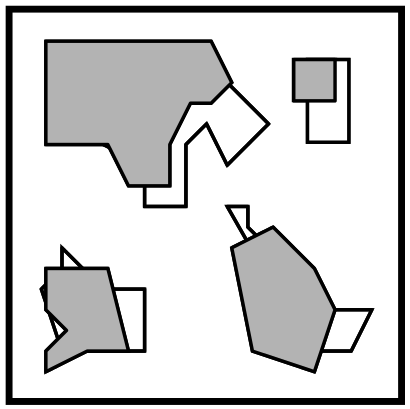
\includegraphics[width=0.4\textwidth]{imagenes/area-e.png}
  \caption{Comparación de espacial.\footfullcite{congalton2008assessing}}
  \end{figure}
\end{frame}
%--- Next Frame ---%

\subsection{Matriz de confusión}
\begin{frame}{\subsecname}
\begin{block}{Definición}
  Lo que esperamos es asignarle a nuestro mapa temático un cierto grado de presición a partir de datos medidos en el terreno.
\end{block}
\end{frame}

\begin{frame}{\subsecname}
\begin{block}{Definición}
\[
\begin{bmatrix}
      & 1               & 2           &  \dots     & k      &  n_{i+}\\
    1 & n_{11}          & n_{12}      & \dots & n_{1k} &  n_{1+}\\
    2 & n_{21}          & n_{22} & \dots & n_{2k} &  n_{2+}\\
    \vdots  & \vdots & \vdots & \ddots      & \vdots         &  \ddots\\
    k & n_{k1} & n_{k2} & \dots       & n_{kk}       &  n_{k+}\\
    n_{+j} & n_{+1} & n_{+2} & \dots & n_{+k} & N
\end{bmatrix} \]
\end{block}
\end{frame}

\begin{frame}{\subsecname}
\begin{block}{Definición}
  Donde
  $$n_{i+} = \sum_j n_{ij}$$
  $$n_{+j} = \sum_i n_{ij}$$
  y donde $n$ es el número total de muestras.
\end{block}
\end{frame}

\begin{frame}{\subsecname}
  \begin{exampleblock}{Ejemplo}
    Vamos a tomar sólo tres coberturas a modo de ejemplo
    \[
    \begin{bmatrix}
          & a   & s    & v  & \\
        a & 50  & 10   & 20 & 80 \\
        s & 5   & 100  & 15 & 120 \\
        v & 10  & 10   & 80 & 100 \\
          & 65  & 120  & 115& 300
    \end{bmatrix} \]
  \end{exampleblock}
\end{frame}

\begin{frame}{\subsecname}
  \begin{block}{Presición total}
    $$O = \sum_i p_{ii}$$
  \end{block}\pause
  \begin{block}{Presición usuario}
    $$U_i = \frac{p_{ii}}{p_{i+}}$$
  \end{block}\pause
  \begin{block}{Presición productor}
    $$P_j = \frac{p_{jj}}{p_{+j}}$$
  \end{block}  \pause
\end{frame}

\begin{frame}{\subsecname}
  \begin{block}{Fracción de la muestra}
      $$p_{ij} = \frac{W_i n_{ij}}{n_{i+}}$$
  \end{block}\pause
  \begin{block}{Probabilidad de j en los datos de campo}
    $$p_{+j} = \sum_i p_{ij}$$
  \end{block}
  \begin{block}{Probabilidad de i en la clasificación}
    $$p_{i+} = \sum_j p_{ij}$$
  \end{block}
\end{frame}

\begin{frame}{\subsecname}
  \begin{exampleblock}{Ejemplo}
      Si las áreas son $A_v = 1000$, $A_a = 500$ y $A_s = 500$ entonces \pause
    \[
    \begin{bmatrix}
          & a   & s        & v    & \\
        a & 0.16  & 0.03   & 0.06 & 0.25 \\
        s & 0.01  & 0.21   & 0.03 & 0.25 \\
        v & 0.05  & 0.05   & 0.40 & 0.50 \\
          & 0.23  & 0.29   & 0.49 & 0.77
    \end{bmatrix} \]
  \end{exampleblock}
\end{frame}

\begin{frame}{\subsecname}
  \begin{block}{Matriz de confusión}
    Cualquier análisis sobre el error de una clasificación parte de la matriz de confusión.
  \end{block}
\end{frame}

\subsection{Estimación de áreas}

\begin{frame}
    \frametitle{\secname-\subsecname}
    \begin{block}{Observación}
        Las áreas podemos estimarlas tanto a partir de $p_{i+}$ y de
        $p_{+j}$.\pause
        \begin{itemize}
            \item $p_{i+}$ se conoce con certeza pero puede estar sesgado.
            \item $p_{+j}$ presenta un sesgo menor pero debe ser estimado.
        \end{itemize}
    \end{block}
\end{frame}

\begin{frame}
    \frametitle{\secname-\subsecname}
    Podemos estimar la varianza de $p_{+j}$ como
    \begin{equation}
        S(p_{+j}) = \sqrt{\frac{W_i p_{ij} - p_{ij}^2}{n_{i+}-1}}
    \end{equation}\pause
    y por lo tanto $$A_k = A_{total} \times p_{+j} \pm 1.96 \times
    A_{total}\times S(p_{+j})$$.
\end{frame}

\begin{frame}
    \frametitle{\secname-\subsecname}
 \begin{exampleblock}{Ejemplo}
     Las áreas con sus errores son
     \begin{itemize}
         \item $A_a = (433\pm88)km^2$
         \item $A_s = (579\pm70)km^2$
         \item $A_v = (988\pm95)km^2$
     \end{itemize}
  \end{exampleblock}
   
\end{frame}

\subsection{Muestreo}

\begin{frame}{\subsecname}
  \begin{block}{4 preguntas}
  \begin{enumerate}
    \item ¿Qué categorías tengo?
    \item ¿Qué unidad de muestreo usar?
    \item ¿Cuántas muestras tomar?
    \item ¿Cómo elegir las muestras?
  \end{enumerate}
  \end{block}
\end{frame}

\begin{frame}{\subsecname}
  \begin{block}{¿Que categorías tengo?}
    Las clases tienen que ser \pause
    \begin{itemize}[<+>]
      \item Mutuamente exclusivas
      \item Totalmente exhaustivas
    \end{itemize}
    Además de tener un tamaño mínimo para ser considerado de esa clase.
  \end{block}
\end{frame}

\begin{frame}{\subsecname}
  \begin{figure}
  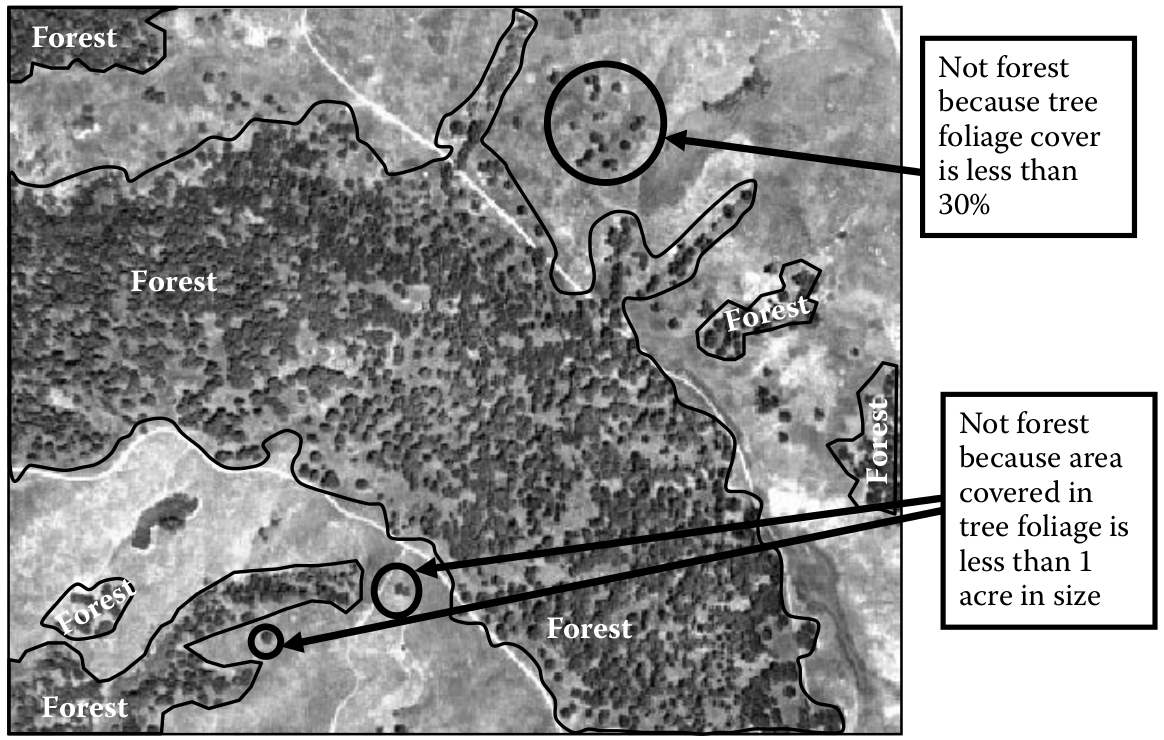
\includegraphics[width=0.8\textwidth]{imagenes/unidad_mapa.png}
  \caption{Clases de muestreo definidas en el terreno.\footfullcite{congalton2008assessing}}
  \end{figure}
\end{frame}
%--- Next Frame ---%

\begin{frame}{\subsecname}
  \begin{block}{¿Qué unidad de muestreo usar?}
    \begin{itemize}[<+>]
      \item Un solo píxel.
      \item Un clúster de píxeles
      \item Un polígono
      \item Un clúster de polígonos
    \end{itemize}
  \end{block}
\end{frame}

\begin{frame}{Muestreo}
  \begin{block}{¿Cuántas muestras tomar?}
    $$N = \frac{B}{4b^2}$$ donde $B$ se obtiene a partir de la distribución $\chi^2$ con un grado de libertad y $b$ es la presición que uno acepta.
  \end{block}
\end{frame}

\begin{frame}{\subsecname}
  \begin{block}{¿Como elegir las muestras?}
    \begin{itemize}[<+>]
      \item Al azar.
      \item Estratificado al azar.
      \item Sistemático.
      \item Clusters
    \end{itemize}
  \end{block}
\end{frame}

\begin{frame}{Muestreo}
  \begin{alertblock}{Logística}
    Todo lo que vimos va a estar supeditado a mi capacidad de realizar el muestreo.
  \end{alertblock}
\end{frame}

\section{Práctica}

\begin{frame}{Práctica}
  \begin{exampleblock}{Actividades prácticas de la sexta clase}
    \begin{enumerate}
      \item Abrir las imágenes clasificadas y fusionadas por el método de clasificación supervisada y no supervisada.
      \item Cargar los polígonos de validación correspondientes a cada clase.
      \item Calcular al matriz de confusión correspondiente a cada clasificación.
      \item Obtener la presición global, del usuario, productor y el índice kappa.
    \end{enumerate}
  \end{exampleblock}
\end{frame}
%--- Next Frame ---%

\end{document}
